\documentclass[a4paper,11pt,dvipdfmx]{jsarticle}

\usepackage{type1cm,newtxtext}
\usepackage{amsmath,amssymb, txfonts}
\usepackage{graphicx}
\usepackage{fancyhdr}
\usepackage{url}
% \usepackage{pxfonts}
\usepackage{framed}

\newcommand{\bm}[1]{\boldsymbol{#1}}

\thispagestyle{fancy}
\lhead{研究会資料}
\rhead{2012.05.08} % 日時を指定する場合
%\rhead{\today} % コンパイル時の日付を入れたい場合


\begin{document}

\begin{center}
\bf \Large
ロボットの研究 %研究題目

\normalsize
槇田 諭 %名前
\end{center}

\pagestyle{fancy}


\section{進捗状況}

研究がとても捗った.


\subsection{具体的にやったこと}

文献\cite{nakamura1990jsice}の理論をもとに,新しいロボットの機構を考案した(\figurename\ref{fig:robot}).
従来のもの\cite{korenara}に比べて3倍の性能をもつ.

\begin{figure}[!b]
\centering
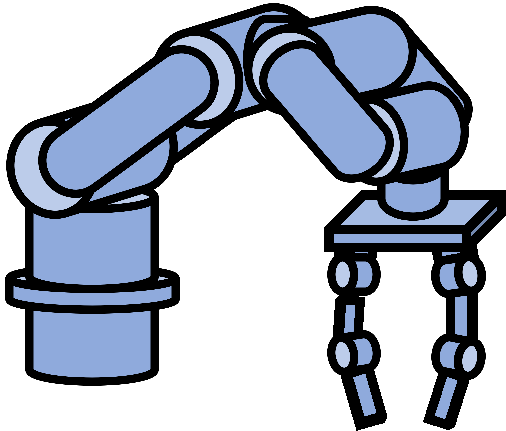
\includegraphics[width=0.4\columnwidth, clip]
 {manipulator-crop.pdf}
\caption{New robot}
\label{fig:robot}
\end{figure}%


\subsection{課題}

新しく考案したロボットの機構は難しすぎて作れない.


\section{今後の予定}

\begin{description}
\item [〜5月31日] 文献調査
\item [6月1日〜] 機構設計
\end{description}

\begin{thebibliography}{9}
\bibitem{nakamura1990jsice}
中村 仁彦:``把持とあやつり'',計測と制御,29巻,3号,pp.|206-212,1990.

\bibitem{korenara}
坪内 孝司,大隅 久,米田 完:
``これならできるロボット創造設計'',
講談社,2007.

\end{thebibliography}

\end{document}